%%
%% LocalControl_CICR.tex
%% Login : <hoang-trong@hoang-trong-laptop>
%% Started on  Thu Jul  9 10:02:35 2009 Hoang-Trong Minh Tuan
%% $Id$
%% 
%% Copyright (C) 2009 Hoang-Trong Minh Tuan
%%

\chapter{Tools and Computational Methods in Cardiac Cell Modelling}
\label{chap:comp-meth-card}

\section{Introduction}
\label{sec:introduction-1}

In deterministic models, the result is interpreted as the average
behavior, as the fluctuations is ignored and assume an isopotential
cell, an approach that is valid for simulating the current flowing
through a large population of Voltage-gated ion channels. 

With the same voltage, identical rate constants can be applied to each
channel, and only the average behavior need to be considered. Such
approach face a drawback as the nature of EC couping process is the
recruitment of thousands of elementary events, known as
{\bf $\ca$ sparks}. This local elevation is the result of the
stochastic interaction of a small number of ion channels in the
so-called dyadic subspace. Each dyadic subspace comprises a small
number of DHPR and RyRs.

It's possible, in principle, to consider all possible ``states'' of
the entire cluster, and determine the transition rates among these
states due to the opening or closing of single channels. However, the
major challenge of this approach is the state space
explosion. Example:
\begin{itemize}
\item With 5 two-state RyR channels, we need $2^5=128$ states, with 50
  two-state RyR channels, we need $2^{50}=1,125,899,906,842,624$
  states. This makes the problem intractable. 


\item An alternate solution to reduce the state space is to assume all
  ion channels are identical. So, we're only interested in how many
  channels in a single state, regardless of the channels
  themselves. This can dramatically reduce the state space, e.g. with
  50 two-state RyRs, we need $\frac{(50+2-1)!}{50!(2-1)!}=50$
  states. If we consider also the DHPR into the clusters, the state
  space may increase up to tens of thousands, which make the state
  transition matrix oversize, e.g. each element is 8 bytes
  (double-precision), then the memory require for a matrix is
  $10000^2\times 8/1024^2 = 762$MB which is pretty big. 


\item One solution, somewhat easier approach, is Monte-Carlo
  simulation, in which stochastic transition of individual channels
  are simulated under the control of pseudo-random numbers. Here, each
  PRN is generated for each channel, then based on comparing this PRN
  with the calculated probability of changing to a new state of each
  channel, the next state of the channel is determined. In an exact
  stochastic simulation, when a single channel is allowed to change at
  a time point, the usage of PRNs are wasted, as tens or hundreds of
  PRNGs are generated when only one is really used. So, this procedure
  is still very intensive computational demand, though not memory
  demand which is better than the two above methods.


\item Another solution is to use probability density approach, under
  the assumption that the amount of CRUs are large enough. 


\item A newer, better solution, known as Ultra-fast Markov-Chain
  Monte-Carlo simulation reduce the memory demands of the second
  method, and improve the third method by using a single PRN for each
  CRU only. 
\end{itemize}

\section{Adaptive time-step}

One of the challenge when running the simulation is tractable in time. Due to
the steepness in some ODE and/or PDE, the time step cannot be too large.
However, the steepness mainly occur when there is action potential (AP). So, a
common approach is using an adaptive time-step, which is large when there's no
many activity and is small when there's an action potential. This is important 
when solving Hodgkin-Huxley type equations of gating variables (e.g. m,h,j for
$I_\na$, r and s for $I_\to$, $x_{r1}$ and $x_{r2}$ for $I_\Kr$; $x_s$ for
$I_\Ks$; d,f and $f_\ca$ for $I_\ca$; $g$ for $I_\rel$).

The main criteria to detect AP is using $dV_m/dt$, the rate of changes of the
membrane potential. \citep{rush1978pas} adjusted the time step from 0.01 to
0.1ms. In particular, step size is 0.01 if $dV_m/dt > 5$mV/ms; otherwise use
step size is $\Delta t=min(0.1, 0.01 \times \frac{5.0}{dV_m/dt})$ ms.

In novel computational model, when gating of individual channels are examined,
the time step should be smaller than 1$\mus$ and can be as small as 10ns; so the
gating variables is not an issue but how to avoid using too small time step; but
having an accurate enough dynamics of individual channel gatings. In such
scenario, stochastic simulation is required as the gating of individual channels
was believed to be random; under the affect of other factors like calcium
concentration or ligand binding which may increase or decrease the affinity of
state transitions. 

\section{Monte-Carlo approach with transient $c_{ds}$}
\label{sec:monte-carlo-approach-1}

Now, there are only $N+2$ ODEs of concentration, instead of $2N+2$ as
being used in the previous model ($N$ is the number of release
sites). The reason is that based on the model parameters, $c^n_{ds}$
reach the equilibrium swiftly and $c^n_{ds}$ is now replaced by
$\overline{c^n_{ds}}$ with
\begin{equation}
  \label{eq:205}
  \overline{c^n_{ds}} =   \overline{c^n_{ds,0}} +  \overline{c^n_{ds,1}}  c_{jsr}
\end{equation}
and 
\begin{equation}
  \label{eq:206}
  \begin{split}
    \overline{c^n_{ds,0}} &= \frac{\gamma^n_{dhpr}J^0_{dhpr} +
      v_{efflux}c_{myo}}{\gamma^n_{ryr} v_{ryr} + v_{efflux} - \gamma^n_{dhpr}J^1_{dhpr}} \\
    \overline{c^n_{ds,1}} &=
    \frac{\gamma^n_{ryr}v_{ryr}}{\gamma^n_{ryr} v_{ryr} + v_{efflux}
      - \gamma^n_{dhpr}J^1_{dhpr}} \\
  \end{split}
\end{equation}
with $J^0_{dhpr}, J^1_{dhpr}$ are functions of plasma membrane voltage
\begin{equation}
  \label{eq:207}
  \begin{split}
    J^0_{dhpr} = \frac{1}{N} \frac{A_mP^T_{dhpr}V}{V_\theta} \left( \frac{c_{ext}}{e^{V/V_\theta}-1}  \right)\\
    J^1_{dhpr} =  -\frac{1}{N} \frac{A_mP^T_{dhpr}V}{V_\theta} \left( \frac{e^{V/V_\theta}}{e^{V/V_\theta}-1}  \right)
  \end{split}
\end{equation}
that satisfy
\begin{equation}
  \label{eq:208}
  J^n_{dhpr} =   \gamma^n_{dhpr} (J^0_{dhpr} + \overline{c^n_{ds}}  J^1_{dhpr})
\end{equation}

\begin{framed}
  In each CaRU, there can be multiple L-type channels and multiple RyR
  channels. However, as the all-or-none model is widely used to study
  the behavior of ion channels, the number of each type of ion channels
  is neglected. As a result, in each release site, it is considered that
  there is one RyR channels and one L-type channel. 
\end{framed}

In this chapter, the 6-state RyR channel and 2-state L-type channel is
utilized. As a result, the number of possible states for a release
site is 12.  With 12-state model (the first index indicates the state
of DHPR, the second index indicates the state of RyR megachannel), we
have a $12\times 12$ infinitesimal generator matrix (Q-matrix). This
matrix is decomposed into three components
\begin{equation}
  \label{eq:209}
  Q = K_\phi(V) + c_{ds}K_{ds} + c_{jsr} K_{jsr}
\end{equation}
with elements of $K_\phi(V)$ are $\Ca$-independents (both
voltage-dependent and voltage-independent, unit: $T^{-1}$). The
elements of $K_{ds}, K_{jsr}$ are the {\it association rate constants
} for the transitions mediated by $c_{ds}$ and $c_{jsr}$, respectively
(unit: concen$^{-1}$.T$^{-1}$). 

The set of ODEs
\begin{eqnarray}
  \label{eq:2300}
  \frac{dc_{myo}}{dt} &&=  J_{leak}+J^T_{efflux} - J_{NCX} - J_{SERCA} +
  J_{in} \\
  \frac{dc_{nsr}}{dt} &&= \frac{1}{\lambda_{nsr}} \left( -J_{leak} +
    J_{SERCA} - J^T_{refill} \right)\\
  \frac{dc^n_{jsr}}{dt} &&= \frac{1}{\lambda_{jsr}} \left( J^n_{refill} -J^n_{ryr} \right)
\end{eqnarray}
\textcolor{red}{Here, we have 12 unknown parameters} 


\section{Deterministic approach}
\label{sec:deterministic_approach}

Hinch et al. \citep{hinch2004mag,hinch2004mag} build an intracellular $\Ca$
models that are computationally minimal but still capture the underlying local
control nature of the process. This can be done by using various asymptotic
timescale reductions and utilizing the law of large numbers (i.e. 20,000 CRUs),
a deterministic model of $\Ca$ release is developed. In this model, the
$Ca$ release in the subspace is assumed to be dependent upon the bulk
NSR $\Ca$, rather than local JSR $\Ca$. This limitation is resolved in
\citep{williams2008mlg} (Sect.\ref{sec:prob-appr}).

This deterministic model was incorporated into a whole-cell model to produce
high gain and graded response \citep{hinch2004slc,greenstein2006}.


\section{Fokker-Planck equation}
\label{sec:Fokker-Planck_equation}

Fokker-Planck equations formally come about by, in loose terms, ``turning a
stochastic differential equation into a partial differential equation (PDE)''.
\textcolor{red}{It is a deterministic PDE describing the evolution of the
probability density function of all molecules's spatial positions}.

In 1D context: let $v(t)$ is a random variable corresponding to the position of
a random-walking particle, with a 'random force' due to collisions
\begin{equation}
m\frac{dv}{dt} = b(v) + \sigma(v) W(t)
\end{equation}
with $b(v), \sigma(v)$ are specified functions of velocity, and $W(t)$ is the
white noise process - an intuitive, but not well-defined, stochastic process
for which $W(t)$ and $W(t+\Delta t)$ are independent $\forall \Delta t \ne 0$.
The second term represents the collisions, which happens at random interval in
time, but with the distribution of the strength of the collision is constant in
time.

Since almost all Brownian motion sample paths are not differentiable at any
time, the white noise process defined in this manner will be ill-defined, as
expected. We can reformulate the equation of motion above in terms of stochastic
differential equation
\begin{equation}
dv = \frac{b(v)}{m}dt + \frac{\sigma(v)}{m} dW(t)
\end{equation}
We can say that: the infinitesimal change in velocity in a time interval $dt$
is proportional to the classical acceleration $d=b(v)/m$ times that time
interval $dt$, plus an extra term which means
we have to slightly change that velocity by a random term.


\citep{risken1997}


\subsection{Model Ca2+ in the dyad}

The motion of a Ca2+ ion in the dyad is influenced by the Brownian random
force from the surrounding solvent and the electrostatic potential stemming
from proteins, membranes, and other ions, including other Ca2+ ions.

Consider $N$ $\Ca$ ions, with join positions represented as 
\begin{equation*}
R = (\mathbf{r}_1, \mathbf{r}_2, \ldots, \mathbf{r}_N)
\end{equation*}
with $\mathbf{r}_i = (x_i,y_i, z_i)$ is a 3D vector. We consider $N$ ions as
a single 'lumped' particle, which can move in a $N$-dimensional space of
Brownian motion.  
The time evolution of this joint probability density of these $\Ca$ ions at position $R$
at time $t$ is
\begin{equation}
P(R,t) = P(\mathbf{r}_1, \mathbf{r}_2, \ldots, \mathbf{r}_N, t)
\end{equation}
which is described by the Fokker-Planck equation (FPE).
The multidimensional FPE describes the evolution of the probability density
function for the position of a Brownian particle subject to a potential $V$
\begin{equation}
\label{eq:fokker-planck}
\frac{\partial P}{\partial t} = D \sum_{i=1}^N \frac{\partial}{\partial
\mathbf{r}_i} \left[  
\frac{1}{k_BT} \frac{\partial V}{\partial \mathbf{r}_i} P(\cdot) +
\frac{\partial P}{\partial \mathbf{r}_i} \right]
\end{equation}
with $D$= diffusion constant, $k_B$= Boltzmann constant, $T$= temperature, 
$V$ = potential energy, and
\begin{equation}
\frac{\partial}{\partial \mathbf{r}_i} = \left(
\frac{\partial}{dx_i}, \frac{\partial}{dy_i}, \frac{\partial}{dz_i}  
\right)
\end{equation}
and the potential energy $V$ of the 'lumped particle' at position $R$ is
\begin{equation}
V(R) = \sum_{i=1}^{N} \left[ 2q \Phi(\mathbf{r}_i) + u(\mathbf{r}_i) \right] +
U(R)
\end{equation}
with $q$ is the elementary charge, and the different contributions are
considered here:
\begin{itemize}
  \item $\Phi(\mathbf{r}_i)$ : electrostatic potential of the $i$-th ion due to
  charges on the surrounding lipids and proteins.

In the dyad, the electrostatic potential is dominated by the membrane surface
charges in the dyad. Here, the Debye-Huckel model of charge-charge interaction 
is used
\begin{equation}
\Phi(\mathbf{r}) = -\Phi_o \int_S \rho(\mathbf{r}')
\frac{e^{-|\mathbf{r}-\mathbf{r'}|/\kappa}}{|\mathbf{r}-\mathbf{r'}}
d\mathbf{r'}
\end{equation}
The integral is taken over the surface area S of the dyad membrane, $\rho$ =
membrane surface charge density, $\kappa$ = Debye length. The constant $\Phi_o$
depends on the dielectric constant and ionic conditions in the dyad.
An apprixmation of this formula is given \citep{soeller1997}
\begin{equation}
\Phi(\mathbf{r}) = -\Phi_{SL} e^{-z/\kappa} - \Phi_{SR} e^{-(h-z)/\kappa}
\end{equation}
with $h$ = height of the dyad, $z$ = vertical distance from the SL at point
$\mathbf{r}$, and $h-z$ = the vertical distance from the SR membrane at point
$\mathbf{r}$.


  \item 
\end{itemize}

Rather than solving the time-dependent joint probability in
eq.\ref{eq:fokker-planck}, a sample path of the $\Ca$ ion movement in the dyad
can be generated using Monte Carlo algorithm \citep{wang2003robust}.

\section{Probabilistic approach}
\label{sec:prob-appr}

Based on a system of Fokker-Planck equations describing the probability density
function (PDF) for the JSR $\Ca$ concentration in the CRU, 
\citep{williams2007pda} proposed a cheaper method to simulate large-scale
Monte-Carlo simulations.

\subsection{Probability approach for a single type of channel}
\label{sec:prob-appr-single}

At first, we examine a single channel.  In general, the activation
rate for a single a single $\Ca$ channel can be either
calcium-dependent, voltage-dependent or both.  For simplicity, we
first examine the diagram for state transition of a two-state single
$\Ca$ channel with the transition rate (in this case it is also
activation rate) is calcium-dependent,
\begin{equation}
  \label{eq:177}
  \ce{C <=>[\ce{k^+ c^\eta}][k^-] O} 
\end{equation}
with $[\text{transition rate}]=$T$^{-1}$ (unit of reciprocal
time). $c$ is the local [$\Ca$]\footnote{the concentration of
  calcium near the $\Ca$-regulated site}. 
\begin{itemize}
\item $k^+$ is the association rate constant with unit
  (concentration$^{-\eta}$ .T$^{-1}$). 
\item $\eta$ is the cooperativity of calcium binding, i.e. denoting
  the number of binding calcium ions required to activate the channel.
\end{itemize}

The state transition above is a discrete-state continuous time
stochastic process that takes on values in the state space
$\mathcal{S} = (C,O)$
(\textcolor{red}{NOTE: the order is important here, as we will use the
  index to denote the state in the programming code},
e.g. 1 for C and 2 for O).  $S(t)$ is used to denote the state of the
channel at the time point $t$.  As the gating is a stochastic process,
$S(t)$ is a random variable . 

If we examine more than one channel, the state spaces would be of
higher dimension, e.g. for three channels
\begin{eqnarray*}
  \mathcal{S}=\{CCC, CCO, COO, COC ... \},
\end{eqnarray*}
yet still a discrete-state continuous time stochastic
process\citep{mazzag2005erca}. Normally, we're only interested in the
number of channels in a particular states. Thus, to make the problem
easier to handle, we define a column-vector whose index referring to a
particular state (that's why we mentioned previously that the order of
the state in the state space is important) and the values of the
corresponding index is the number of channels in that state. 

Example: for a single channel with two states, we have
$\mathbf{u}_0=[0,1]^T$ or $\mathbf{u}_0=[1,0]^T$. In the more
complicated situation, i.e. more than two states or more than one
channels, a combinatoric arrangements should be identified. For
example, for 3 states and 2 channels
\begin{verbatim}
st1 st2 st3
 2   0   0
 1   1   0
 1   0   1
 0   2   0
 0   1   1
 0   0   2
\end{verbatim}

% If we examine more than one type of channel, the state spaces would be
% of higher dimension, e.g. for two types of channels
% \begin{eqnarray*}
%   \mathcal{S}=\{C_1C_2, C_1O_2, O_1O_2, O_1C_2\},
% \end{eqnarray*}
% yet still a discrete-state continuous time stochastic
% process\citep{mazzag2005erca}. If we examine a CaRU, this state space
% will be explosive as we may have a bunch of channels for each
% type. Thus,
% \textcolor{red}{we will learn using algebraic representation (matrix,
%   vector) to represent the states}.


\subsection{Assumptions}
\label{sec:assumptions}


Paper: ~\citep{williams2007pda}.

Assumption: there is a large number $N$ of CaRUs. $N=20,000$ CaRU are
used to model the stochastic gating.  In this paper,
\textcolor{red}{all-or-none manner is assumed, i.e. each CaRU has only
  one RyR megachannel, and one L-type channel}.

In this paper, for the purpose of validating the probability density
approach which is being introduced in the next section, the Markov
model of reduced complexity is used, i.e. minimal whole cell model
with each channel has 2 states.

% minimal model = the most basic model
{\bf Minimal model for a single RyR channel:}
\begin{equation}
  \label{eq:161}
C \ce{<=>[k^+_{ryr}(c^n_{ds},c^n_{jsr})][k^-_{ryr}]} O  
\end{equation}
with the activation {\it rate constant} is calcium ($c_{ds}$ and
$c_{jsr}$) dependent, and the inactivation $k^-_{dhpr}$ is assumed to
be a constant.

{\bf Minimal model for a single L-type $\Ca$-channels}
\begin{equation}
  \label{eq:162}
C \ce{<=>[k^+_{dhpr}(V)][k^-_{dhpr}]} O    
\end{equation}
with the activation is voltage-dependent and the inactivation
$k^-_{ryr}$ is assumed to be a constant.

Finally,
\textcolor{red}{each  CaRU is modelled as a 4-state release
  site} ($M = 4$).
\begin{equation}
  \label{eq:163}
  \begin{array}{c}
      CC \ce{<=>[k^+_{ryr}(c^n_{ds},c^n_{jsr})][k^-_{ryr}]} CO \\
        k^+_{dhpr}(V) \Updownarrow  k^-_{dhpr}   
        \text{\hspace{10 mm}     } k^-_{dhpr} \Updownarrow  k^+_{dhpr}(V)  \\
      OC \ce{<=>[k^-_{ryr}][k^+_{ryr}(c^n_{ds},c^n_{jsr})]}OO\\
  \end{array}
\end{equation}

\subsection{Values for inactivation rates}
\label{sec:valu-inact-rates}

Both $k^-_{dhpr}$ and $k^-_{ryr}$ are chosen as fixed values so that
the mean open-time is 0.2ms and maximum open probability is 0.1 for
L-type $\Ca$-channel and RyR channels, respectively.
\begin{equation}
  \label{eq:167}
  \begin{split}
      k^-_{dhpr} &= constant \\
      k^-_{ryr} &= constant \\      
  \end{split}
\end{equation}

\subsection{Values for activation rates}
\label{sec:valu-activ-rates}

The rate constant for the activation of the cluster of RyR is a
sigmoidal function of the dyadic subspace
[$\Ca$]\citep{sobie2002tcas}.
\begin{equation}
  \label{eq:164}
  k^+_{ryr} = \overline{k^+_{ryr}} \frac{(c^n_{ds})^4}{(K_{ryr})^4 + (c^n_{ds})^4}
\end{equation}
with $\overline{k^+_{ryr}}$ is the maximum value, $K_{ryr}$ is
half-maximal activation of RyR megachannel, a decreasing function of $c^n_{jsr}$.  
\begin{equation}
  \label{eq:166}
  K_{ryr} = K^{max}_{ryr} - \alpha_{ryr} c^n_{jsr}
\end{equation}

The rate constant for the activation of the L-type \ce{Ca^2}-channels
is\citep{luo1994dmc_b}.
\begin{equation}
  \label{eq:165}
  k^+_{dhpr} = \overline{k^+_{dhpr}} \frac{e^{(V_m -
      V^\theta_{dhpr})/\sigma_{dhpr}}}{1+e^{(V_m -
      V^\theta_{dhpr})/\sigma_{dhpr}} }
\end{equation}
with $ \overline{k^+_{dhpr}}$ is the maximum value, $V_m$ is the
membrane potential, $V^\theta_{dhpr}$ is the reversible potential.


{\bf Assumption}: 
\begin{enumerate}
\item It ignores the voltage- and $\Ca$-dependent of the
  inactivation rate $k^-_{dhpr}$.
\item Two-state DHPR model and two-state RyR model
\item All-or-none behavior of DHPR and RyR channels $==>$ CaRU is
  modelled as a 4-stage release site.
\end{enumerate}

{\bf Target}: Model the triggering of CICR during the whole-cell
voltage clamp protocols.

\subsubsection{Algebraic representation}
\label{sec:algebr-repr}

All rate transitions in the state space for the dichotomous situation
above can be represented using the idea of the famous
{\bf telegraph process} is
used\footnote{\url{http://en.wikipedia.org/wiki/Telegraph_process}}.
This is a memoryless continuous-time stochastic process,
% At a given time instance, the local [$\Ca$] is constant,
% e.g. equal to the fixed background [$\Ca$] denoted by $c_\infty$,
then the {\it Q-matrix} (the infinitesimal matrix) of that process is
\begin{equation}
\label{eq:179}
  Q = (q_{ij}) = \left( 
    \begin{array}{cc}
      -k^+c^\eta & k^+c^\eta\\
      k^- & -k^-\\
    \end{array}
\right)
\end{equation}
The off-diagonal elements $q_{ij}$ ($i\ne j$) of the infinitesimal
generator matrix (Q-matrix) is itself the transition rate (i.e. the
probability) from state $i$-th to state $j$-th per unit time.
\begin{equation}
  \label{eq:181}
  q_{ij} = \lim_{\Delta \rightarrow 0} \frac{Prob[S(t+\Delta t) = \mathcal{S}_j| S(t)
    =\mathcal{S}_i ]}{\Delta t}
\end{equation}

For easier manipulation in programming, this Q-matrix can be
decomposed into two separate matrices $K_-$ and $K_+$ (or some others
use $K_m$ and $K_p$ with $m=minus, p=plus$).
\begin{equation}
  \label{eq:180}
  Q =  \left( 
    \begin{array}{cc}
      0 & 0\\
      k^- & -k^-\\
    \end{array}
\right) + c^\eta  \left( 
    \begin{array}{cc}
     -k^+ & k^+\\
     0 & 0\\
    \end{array}
\right)
\end{equation}
with
\begin{equation}
  \label{eq:388}
K_m =  \left( 
    \begin{array}{cc}
      0 & 0\\
      k^- & -k^-\\
    \end{array}
\right); \; K_p =  \left( 
    \begin{array}{cc}
     -k^+ & k^+\\
     0 & 0\\
    \end{array}
\right)  
\end{equation}

Now, we examine the $\Ca$-inactivation process.
\begin{equation}
  \label{eq:193}
   \ce{O <=>[\ce{k^+ c^\eta}][k^-] C}
\end{equation}
In this situation, the Q-matrix would be the same if we invert the
order of the states, i.e. (1,2) = (O,C)=$\mathcal{S}$.

% To make the problem easier to handle, we define a column-vector whose
% elements are 1 if the channel is open, and 0 otherwise. Thus, for the
% $\Ca$-activated process, $\mathbf{u}_0=[0,1]^T$; while for the
% $\Ca$-inactivated process, $\mathbf{u}_0=[1,0]^T$. In the more
% complicated situation, e.g. more than two states, a combinatoric
% arrangements should be identified, e.g. for 3 states and 3 channels


% \begin{verbatim}
% 2 0 0 

% \end{verbatim}

However, due to the effect of the residual $\Ca$ on
channels~\citep{mazzag2005erca}, the local [$\Ca$] will generally
not be given the constant values, but rather decrease or increase
depending on the channels are closed or open. Thus, although the
stochastic process given by $S(t)$, and $c(t)$ has the Markov
property, the Markov chain $S(t)$ is {\it time-inhomogeneous} as the
transition rate is not constant but rather functions of time.

\subsection{Probability approach for CaRU model - bivariate}
\label{sec:prob-appr-caru-1}

In the previous section, we described the probability approach of a
single type of ion channel. As single CaRU has two types of ion
channels, there is an important difference we need to discriminate:
the state of a single channel and the state of a release site. Thus,
in general, we need two vectors $U_R, U_L$, whose elements are vectors
of denoting the state of the release site, i.e. $u_{R,i}$ is the
vector whose elements $u_{R,i}[j]$ denoting the number of L-type
channels in the state $j$ of L-type, $v_{R,i}$ is the vector whose
elements $u_{L,i}[j]$ denoting the number of RyR channels in the state
$j$ of RyR.

When the number of CaRU is large, then the selection of a single CaRU
can be considered as a random process. The state space $\mathcal{S}$
of a release site, as described in the previous section, is dependent
on the number of states of a single type of channel, and the number of
channels for each type. For validation of the method, i.e. the
probability approach, the minimum whole cell model and the all-or-none
behavior of RyR megachannel, as well as DHPR channel, was
assumed. Under that assumption, the state space of one CaRU is
$\mathcal{S} = \{CC, CO, OO, OC\}$ with 4 elements. The first index of
a state is the state of DHPR, the second index of a state is the state
of RyR.

If there is a large number of CaRUs, then at any time $t$, one could
randomly sample one CaRU from the population to produce an instance of
the random variables $\tilde{S}(t)$. To make it complete, we need to
define a measure on $\tilde{S}(t)$, i.e. the probability
distribution. Based on the model described in the previous section, a
state of a CaRU is determined by two concentrations ($c^n_{jsr},
c^n_{ds}$) with $n$ is a randomly selected index. As the
concentrations, denoted by $\tilde{c}_{ds}(t), \tilde{c}_{jsr}(t)$ are
continuous random variables, their instances are denoted by
$[c_{ds},c_{ds}+dc_{ds}],[c_{jsr}, c_{jsr}+dc_{jsr}]$, respectively.

As a result, the gating mechanism can be represented using a
probability density function conditioned on its state. This is a
continuous multivariate probability density functions of both the
$\Ca$ concentrations in dyadic subspace ($\tilde{c}_{ds}(t)$) and
junctional SR ($ \tilde{c}_{jsr}(t)$) given its state, at time $t$, is $i$.
% Finally, the probability to select a CaRU and its the state is $i$ at a time
% point $t$ is the
% for 
% , that
% is
%   \begin{multline}
%     \label{eq:195}
%       \rho^i(c_{ds},c_{jsr},t) dc_{ds}dc_{jsr} =&
%   Prob((c_{ds}<\tilde{c}_{ds}(t) < c_{ds} + dc_{ds}) \cap \\
%     &(c_{jsr}<\tilde{c}_{jsr}(t) < c_{jsr} + dc_{jsr}) \cap \\
%     &\tilde{S}(t)=i )
%   \end{multline}

\begin{eqnarray*}
  \rho^i(c_{ds},c_{jsr},t) dc_{ds}dc_{jsr} =&
  Prob((c_{ds}<\tilde{c}_{ds}(t) < c_{ds} + dc_{ds}) \cap \\
  &(c_{jsr}<\tilde{c}_{jsr}(t) < c_{jsr} + dc_{jsr}) \cap \\
  &\tilde{S}(t)=i )
\end{eqnarray*}

{\bf TIPS}: The index for the state of a CaRU is denoted by $i$ ($1\le
i \le M$), while $n$ is the index for a CaRU ($1 \le n \le N$). In the
probability density approach, $N$ is no longer used.

There are totally $M=4$ probability density functions to examine.
Now, we study the dynamics, i.e. the change, in these
density functions. The change in probability at a particular states are
due to (1) the change in state ($i$ to $j$) (reaction), (2) the change in
concentration $c_{ds}, c_{jsr}$ (advection diffusion).

Let's break down the situation.
\begin{itemize}
\item If the current state is CC (the first C is the state of DHPR and
  the second C is the state of RyR), then the next possible state is
  CO or OC. Given that
  \begin{equation}
    \label{eq:194}
    \begin{split}
       C \ce{<=>[k^+_{dhpr}][k^-_{dhpr}]} O;      C \ce{<=>[k^+_{ryr}][k^-_{ryr}]} O 
    \end{split}
  \end{equation}

  The probability of state transition for CC, thus, is denoted by
  \begin{equation}
    \label{eq:197}
    k^-_{ryr}\rho^{CO} + k^-_{dhpr} \rho^{OC} - (k^+_{dhpr}+k^+_{ryr})\rho^{CC}
  \end{equation}

\item If the decrease in concentration is represented by the {\bf advection
  rate} $f^i_{ds}, f^i_{jsr}$. Thus, the downward change in
  concentration has the negative effect on the probability.  We take
  the example for the case of CC state
  \begin{equation}
    \label{eq:198}
    -\frac{\partial}{\partial c_{ds}}[f^{CC}_{ds}\rho^{CC}] -\frac{\partial}{\partial c_{jsr}}[f^{CC}_{jsr}\rho^{CC}]
  \end{equation}
\end{itemize}

For this multivariate probability density to be consistent with the
dynamics of the Monte Carlo model of cardiac EC coupling, in essence,
the change in 4 probability density functions are represented by a set
of four advection-reaction equations (note the first index is DHPR)
\begin{equation}
  \label{eq:196}
  \begin{split}
    \frac{\partial \rho^{CC}}{\partial t} &=   -\frac{\partial}{\partial  c_{ds}}[f^{CC}_{ds}\rho^{CC}] -\frac{\partial}{\partial
    c_{jsr}}[f^{CC}_{jsr}\rho^{CC}] + k^-_{ryr}\rho^{CO} + k^-_{dhpr} \rho^{OC} - (k^+_{dhpr}+k^+_{ryr})\rho^{CC} \\ 
  \frac{\partial \rho^{CO}}{\partial t} &=  -\frac{\partial}{\partial  c_{ds}}[f^{CO}_{ds}\rho^{CO}] -\frac{\partial}{\partial
    c_{jsr}}[f^{CO}_{jsr}\rho^{CO}] + k^-_{ryr}\rho^{CC} + k^-_{dhpr}
  \rho^{OO} - (k^+_{dhpr}+k^+_{ryr}) \rho^{CO} \\
  \frac{\partial \rho^{OO}}{\partial t} &= -\frac{\partial}{\partial  c_{ds}}[f^{OO}_{ds}\rho^{OO}] -\frac{\partial}{\partial
    c_{jsr}}[f^{OO}_{jsr}\rho^{OO}] + k^-_{ryr}\rho^{OC} + k^-_{dhpr}
  \rho^{CO} - (k^+_{dhpr}+k^+_{ryr}) \rho^{OO}   \\
  \frac{\partial \rho^{OC}}{\partial t} &=  -\frac{\partial}{\partial  c_{ds}}[f^{OC}_{ds}\rho^{OC}] -\frac{\partial}{\partial
    c_{jsr}}[f^{OC}_{jsr}\rho^{OC}] + k^-_{ryr}\rho^{OO} + k^-_{dhpr}
  \rho^{CC} - (k^+_{dhpr}+k^+_{ryr}) \rho^{OC}  
  \end{split}
\end{equation}
\textcolor{red}{Here we have total 8 unknown parameters,} $f^i_{ds},
f^i_{jsr}$ ($i=\overline{1..4}$).

Noting that this can be compactly represented using matrix form
\begin{equation}
  \label{eq:204}
  \frac{\partial \rho^i}{\partial t} = - \frac{\partial}{\partial
    c_{ds}}[f^i_{ds}\rho^i] - \frac{\partial}{\partial
    c_{jsr}}[f^i_{jsr}\rho^i]  + [Q\rho]^i
\end{equation}
with $[\rho Q]^i$ is the $i$-th element of the vector-matrix
multiplication $ Q\rho$ (size: $M\times 1$).  The infinitesimal generator matrix (Q-matrix) is
\begin{equation}
  \label{eq:211}
  \begin{array}{ccccc}
         & CC & CO & OO & OC \\
     CC  & -(k^+_{ryr}+k^+_{dhpr}) & k^+_{ryr}  & 0  & k^+_{dhpr} \\
     CO  &  k^-_{ryr} & -(k^-_{ryr} +k^+_{dhpr})  & k^+_{dhpr} & 0\\
     OO   & 0 & k^-_{dhpr} &-(k^-_{dhpr}+k^-_{ryr} )  & k^-_{ryr} \\
     OC   & k^-_{dhpr}  & 0 & k^+_{ryr} & -(k^-_{dhpr}+k^+_{ryr}) \\
  \end{array}
\end{equation}
{\bf TIPS}: Note the special characteristic of this matrix - the sum
of elements on each row is zero.

Finally, we use the notation $\rho$ as a column-vector
\begin{equation}
  \label{eq:212}
  \rho = \left[
    \begin{array}{c}
      \rho^{CC} \\
      \rho^{CO} \\
      \rho^{OO} \\
      \rho^{OC}
    \end{array}
    \right]
\end{equation}


{\bf idenfity 8} with the advection rates are functions of $c_{ds},
c_{jsr}$
\begin{equation}
  \label{eq:200}
  \begin{split}
      f^i_{ds} &= \frac{1}{\lambda^T_{ds}} \left( \gamma^i_{dhpr}J^T_{dhpr}
      + \gamma^i_{ryr}J^T_{ryr} - J^T_{efflux}  \right) \\
  f^i_{jsr} &= \frac{1}{\lambda^T_{jsr}} \left(J^T_{refill}
      - \gamma^i_{ryr}J^T_{ryr}  \right) 
  \end{split}
\end{equation}
with $\gamma^T_{ds} = N\gamma_{ds}$, $\gamma^T_{jsr} =
N\gamma_{jsr}$. In these 8 equations, we have 4 unknown fluxes.  The
four fluxes that may influences the dyadic subspace and junctional SR
are
\begin{eqnarray*}
  J^T_{ryr} &= v^T_{ryr} (c_{jsr} - c_{ds})\\
  J^T_{efflux} &= v^T_{efflux} (c_{ds} - c_{myo}(t)) \\
  J^T_{refill} &= v^T_{refill} (c_{nsr}(t) - c_{jsr}) \\
  J^T_{dhpr} &= -A_m P^T_{dhpr} \frac{V}{V_\theta} \left( \frac{c^n_{ds}e^{V/V_\theta}-c_{ext}}{e^{V/V_\theta}-1}  \right) 
\end{eqnarray*}
These equations involve the two dynamics quantities [$\Ca$] of bulk myoplasmic ($c_{myo}(t)$) and
network SR ($c_{nsr}(t)$) are time-variant quantities which satisfy the ODEs
\begin{eqnarray*}
  \frac{dc_{myo}}{dt} &= J_{leak} + J^*_{efflux} - J_{NCX} - J_{SERCA}
  + J_{in} \\
  \frac{dc_{nsr}}{dt} &= \frac{1}{\lambda_{nsr}} (J_{SERCA} -  J^*_{refill} - J_{leak})
\end{eqnarray*}
with $J_{leak}, J_{SERCA}, J_{in}$ are determined using the equations
in the Monte Carlo approach. The only difference is with the
$J^*_{efflux}$ and $J^*_{refill}$ which are the function of $c_{ds}$
and $c_{jsr}$. In other words, they are functional form of the
probability densities
\begin{eqnarray*}
  J^*_{efflux} = \int^\infty_0 \int^\infty_0 v^T_{efflux} \left[ c_{ds}
    - c_{myo}(t)  \right] \rho^T(c_{ds},c_{jsr}, t)dc_{ds}dc_{jsr}\\
  J^*_{refill} =  \int^\infty_0 \int^\infty_0 v^T_{refill} \left[ c_{nsr}(t)
    - c_{jsr}  \right] \rho^T(c_{ds},c_{jsr}, t)dc_{ds}dc_{jsr}
\end{eqnarray*}
where $\rho^T(c_{ds},c_{jsr},t) = \sum_{i=1}^M \rho^i$ is the total
probability distribution of the dyadic subspace and junctional SR
irrespective of the state of a randomly sampled CaRU.

The probability density approach produce the distribution of
[$\Ca$] in (1) dyadic subspace and (2) junctional SR based on a
system of partial differential equations, eq.~\eqref{eq:196}.

\subsection{Validate the model}
\label{sec:validate-model}

To validate the novel probability density approach, traditional Monte
Carlo simulation of graded, locally controlled SR $\Ca$ release
is utilized.

\subsubsection{MC simulations}
\label{sec:mc-simulations}

Solving $2+2N$ ODEs, applying the holding potential of $-80$mV
followed by 20ms duration of test potential $-30, -20, -10$ mV. The
$\Ca$ release exhibited by this MC model is graded with changes
in membrane potential and depolarization duration, the phenomena that
are not observed in the common-pool model of EC coupling.



In MC approach, $2N+2$ ODEs are solved to determine the dynamics of
[$\Ca$] in the dyadic subspace and junctional SR associated with
$N$ CaRUs. In probability density approach, the time-dependent
bivariate probabilities are updated using 4 ODEs. The number of ODEs
in the later approach is equal to the number of states of a CaRU.


..............

\subsection{Analysis the dynamics of a CaRU}
\label{sec:analys-dynam-caru}

In the previous probability density approach, 4 ODEs of
advection-reaction equations are solved numerically. As shown in
Fig.~\ref{fig:Ca_ds_jsr}, when the DHPR initially open ($CC-->OC$), an
influx of trigger $\Ca$ leads to $\approx 7\mu$M in $c_{ds}$ and
causes the RyR cluster to open ($OC-->OO$). The resulting CICR
mechanism quickly drives the $c_{ds}$ to $\approx 150\mu$M. Note that
the junctional SR depletion is nearly complete ($c_{jsr}\approx 0$)
before the $CO-->CC$ transition to complete the CICR cycle. 

\begin{figure}[hbt]
 \centerline{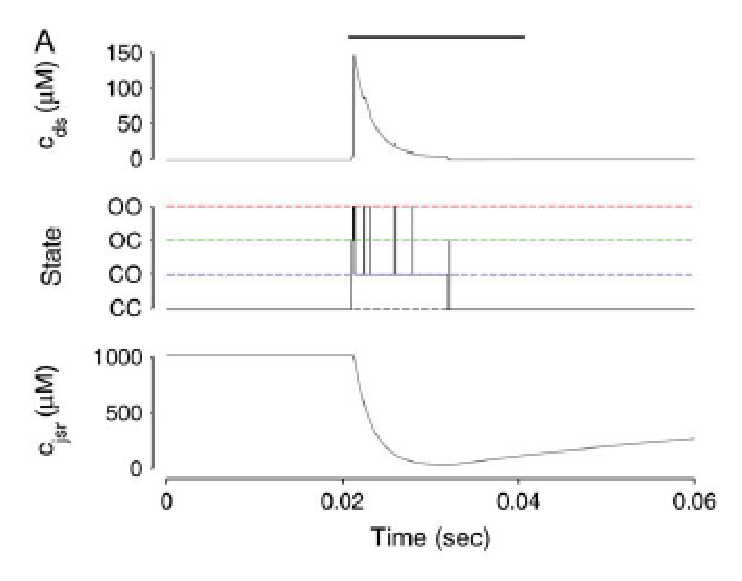
\includegraphics[height=5cm]{./images/Ca_ds_jsr.eps}}
\caption{The dynamics of [$\Ca$] in dyadic subspace and
  junctional SR}
\label{fig:Ca_ds_jsr}
\end{figure}

The dynamics of $c^n_{ds}$ is much faster than that of $c^n_{jsr}$, as
shown in Fig.~\ref{fig:Ca_ds_jsr}. Thus, based on the model
parameters, $c^n_{ds}$ reach the equilibrium swiftly or
\begin{equation}
  \label{eq:210}
  dc^n_{ds}/dt  = 0
\end{equation}
Substituting this equation to the left side of eq.~\eqref{eq:183}, the
solution is
\begin{equation}
  \label{eq:220}
  \overline{c^n_{ds}} = \frac{\gamma^n_{dhpr}J^0_{dhpr}+v^T_{efflux}c_{myo}+\gamma^n_{ryr}v^T_{ryr}c^n_{jsr}}{\gamma^n_{ryr} v^T_{ryr} + v^T_{efflux}
      - \gamma^n_{dhpr}J^1_{dhpr}}
\end{equation}
with $J^0_{dhpr}, J^1_{dhpr}$ are functions of plasma membrane voltage
\begin{equation}
  \label{eq:221}
    \begin{split}
    J^0_{dhpr} = \frac{1}{N} \frac{A_mP^T_{dhpr}V}{V_\theta} \left( \frac{c_{ext}}{e^{V/V_\theta}-1}  \right)\\
    J^1_{dhpr} =  -\frac{1}{N} \frac{A_mP^T_{dhpr}V}{V_\theta} \left( \frac{e^{V/V_\theta}}{e^{V/V_\theta}-1}  \right)
  \end{split}
\end{equation}
that satisfy
\begin{equation}
  \label{eq:2082}
  J^n_{dhpr} =   \gamma^n_{dhpr} (J^0_{dhpr} + \overline{c^n_{ds}}  J^1_{dhpr})
\end{equation}

The solution is split into 2 components (calcium-independent and
$c_{jsr}$-dependent):
\begin{equation}
  \label{eq:2051}
  \overline{c^n_{ds}} =   \overline{c^n_{ds,0}} +  \overline{c^n_{ds,1}}  c_{jsr}
\end{equation}
with
\begin{equation}
  \label{eq:2061}
  \begin{split}
      \overline{c^n_{ds,0}} &= \frac{\gamma^n_{dhpr}J^0_{dhpr} +
        v_{efflux}c_{myo}}{\gamma^n_{ryr} v_{ryr} + v_{efflux} - \gamma^n_{dhpr}J^1_{dhpr}} \\
      \overline{c^n_{ds,1}} &=
      \frac{\gamma^n_{ryr}v_{ryr}}{\gamma^n_{ryr} v_{ryr} + v_{efflux}
      - \gamma^n_{dhpr}J^1_{dhpr}} \\
  \end{split}
\end{equation}


\subsection{Probability approach for CaRU model - univariate}
\label{sec:prob-appr-caru}

Based on the previous analysis, it is inferred that at a given state
$i$, the concentration of $\Ca$ at the dyadic subspace will be at
equilibrium. In other words, $c_{ds}$ at state $i$ is
$\overline{c}^i_{ds}$. 
\begin{equation}
  \label{eq:223}
   \overline{c^i_{ds}} = \frac{\gamma^i_{dhpr}J^0_{dhpr}+v^T_{efflux}c_{myo}+\gamma^i_{ryr}v^T_{ryr}c_{jsr}}{\gamma^i_{ryr} v^T_{ryr} + v^T_{efflux}
      - \gamma^i_{dhpr}J^1_{dhpr}}
\end{equation}
is the function of $c_{myo}(t), c_{jsr}$ and CaRU state $i$.

Correspondingly, the bivariate probability density function can be
well approximated by a univariate probability density function
\begin{equation}
  \label{eq:222}
  \rho^i(c_{ds},c_{jsr},t) = \rho^i(c_{jsr},t)\delta(c_{ds}-\overline{c^i_{ds}})
\end{equation}
with $\delta$ is the unit delta function and
\begin{equation}
  \label{eq:224}
     \rho^i(c_{jsr},t) dc_{jsr} =  Prob \left((c_{jsr}<\tilde{c}_{jsr}(t) <
    c_{jsr} + dc_{jsr}) \text{ and } \tilde{S}(t)=i \right)
\end{equation}
Finally, the resulting advection-reaction equations are
\begin{equation}
  \label{eq:225}
    \begin{split}
    \frac{\partial \rho^{CC}}{\partial t} &=   -\frac{\partial}{\partial
    c_{jsr}}[\overline{f}^{CC}_{jsr}\rho^{CC}] + k^-_{ryr}\rho^{CO} + k^-_{dhpr} \rho^{OC} - (k^+_{dhpr}+k^+_{ryr})\rho^{CC} \\ 
  \frac{\partial \rho^{CO}}{\partial t} &=  -\frac{\partial}{\partial
    c_{jsr}}[\overline{f}^{CO}_{jsr}\rho^{CO}] + k^-_{ryr}\rho^{CC} + k^-_{dhpr}
  \rho^{OO} - (k^+_{dhpr}+k^+_{ryr}) \rho^{CO} \\
  \frac{\partial \rho^{OO}}{\partial t} &= -\frac{\partial}{\partial
    c_{jsr}}[\overline{f}^{OO}_{jsr}\rho^{OO}] + k^-_{ryr}\rho^{OC} + k^-_{dhpr}
  \rho^{CO} - (k^+_{dhpr}+k^+_{ryr}) \rho^{OO}   \\
  \frac{\partial \rho^{OC}}{\partial t} &=  -\frac{\partial}{\partial
    c_{jsr}}[\overline{f}^{OC}_{jsr}\rho^{OC}] + k^-_{ryr}\rho^{OO} + k^-_{dhpr}
  \rho^{CC} - (k^+_{dhpr}+k^+_{ryr}) \rho^{OC}  
  \end{split}
\end{equation}
\textcolor{red}{Here, we have only 4 unknown parameters} $\overline{f}^i$ ($i=\overline{1..4}$), and $\rho^i
= \rho^i_{jsr}$, and
\begin{equation}
  \label{eq:226}
  \begin{split}
      \overline{f^i_{jsr}} &= \frac{1}{\lambda^T_{jsr}}
  (J^T_{refill}-\gamma^i_{ryr}J^T_{ryr}) \\
  &=  \frac{1}{\lambda^T_{jsr}}
  (v^T_{refill} (c_{nsr}(t)-c_{jsr})-\gamma^i_{ryr}v^T_{ryr}(c_{jsr}-\overline{c^i_{ds}}(t)))
  \end{split}
\end{equation}
Here, $c_{myo}$ and $c_{nsr}$ are time-variant quantities and thus we
need to define two ODEs which is similar to those of the previous
section. Other parameters are derived similarly to the previous
approach, except for the two quantities
\begin{equation}
  \label{eq:234}
  \begin{split}
  J^*_{efflux} = \sum_{i=1}^M \int^\infty_0 v^T_{efflux} \left[ \overline{c}^i_{ds}
    - c_{myo}(t)  \right] \rho^T(c_{ds},c_{jsr}, t)dc_{ds}dc_{jsr}\\
  J^*_{refill} = \sum_{i=1}^M \int^\infty_0 v^T_{refill} \left[ c_{nsr}(t)
    - c_{jsr}  \right] \rho^T(c_{ds},c_{jsr}, t)dc_{ds}dc_{jsr}
\
  \end{split}
\end{equation}

The fraction of CaRU in each state at a given time $t$ is
\begin{equation}
  \label{eq:235}
  \pi^i(t) = Pr{\tilde{S}(t) = i} = \int_0^\infty \rho^i_{jsr}(c_{jsr},t)dc_{jsr}
\end{equation}

\section{Moment closure}
\label{sec:moment-closure}

The previous chapter simulates the triggering of CICR in cardiac cells
using the probability density approach. This is the continuous work
from that chapter\citep{williams2008mclc} based on the observed fast
characteristic of the $c_{ds}$ compared to the $c_{jsr}$. In other
words, the univariate probability density is utilized and such
distribution is studied under the view points of its moments. Hence,
understanding local control theory
(Sect. \ref{sec:cru_calcium_release_unit}) is recommended.


As mentioned in the previous chapter, when the dynamic of subspace
[$\Ca$] are much faster than those of junctional SR [$\Ca$],
[$\Ca$] in the dyadic subspace are assumed to be quasistatic
equilibrium.  This assumption is utilized to study the moment closure
using probability density approach. In essence, the paper study the
time-dependent univariate density distribution of the [$\Ca$] in
junctional SR ($c_{jsr}$) conditioned on CaRU state by examining its
moments (zero-th, first, and second-order).


{\bf Assumption}: There is some changes compared with the previous
model:
\begin{enumerate}
\item dynamic of subspace [$\Ca$] are much faster than those of
  junctional SR [$\Ca$] $==>$ rapid equilibration of the dyadic
  subspace in each CaRU
\item 2-state for DHPR and 6-state for RyR

\item all-or-none behavior of RyR and DHPR  $==>$ twelve-state CaRU
  model is examined.
  \begin{equation}
    \label{eq:201}
    C_1  \ce{<=>[4k^+_{ryr}][\beta^3k^-_{ryr}]} C_2
    \ce{<=>[3\alpha k^+_{ryr}][2\beta^2k^-_{ryr}]} C_3
    \ce{<=>[2\alpha^2k^+_{ryr}][3\beta k^-_{ryr}]} C_4
    \ce{<=>[k^+_{ryr}][4k^-_{ryr}]} C_5
    \ce{<=>[k^+_{ryr}][k^-_{ryr,*}]} O
  \end{equation}
\end{enumerate}



\subsection{Probability approach with transient $c_{ds}$}
\label{sec:prob-appr-moment}

In the previous chapter, it is inferred that when the calcium
concentration in dyadic subspace are observed to reach quasitatic
equilibrium rapidly, the bivariate probability density model
$\rho^i(c_{ds},c_{jsr},t) dc_{ds}dc_{jsr}$ can be reduced to the
univariate one $\rho^i(c_{jsr},t)dc_{jsr}$ with $1 \le i \le M$,
$M=12$ is the number of states in a release site (aka
cluster-state). In essence, we have a univariate probability density
model.
\begin{equation}
  \label{eq:202}
  \rho^i(c_{jsr},t) dc_{jsr} =  Prob \left((c_{jsr}<\tilde{c}_{jsr}(t) <
    c_{jsr} + dc_{jsr}) \text{ and } \tilde{S}(t)=i \right)
\end{equation}

The change of these $M=12$ probability density functions are
consistent with the dynamics of the Monte Carlo model of EC coupling
as $N\rightarrow \infty$ and as the result, the set of
advection-reaction equations now is (as $f^i_{ds}=0$)
\begin{equation}
  \label{eq:203}
  \frac{\partial \rho^{i}}{\partial t} = -\frac{\partial}{\partial
    c_{jsr}}[f^{i}_{jsr}\rho^{i}] + [Q\rho ]^i
\end{equation}
$Q$ is the $M \times M$ generator matrix, with
\begin{equation}
  \label{eq:213}
  \begin{split}
    f^i_{jsr} &= \frac{1}{\lambda^T_{jsr}} \left(J^T_{refill}
      - \gamma^i_{ryr}J^T_{ryr}  \right)  \\
    &=  \frac{1}{\lambda^T_{jsr}} \left(v^T_{refill}(c_{nsr}-c^i_{jsr})
      - \gamma^i_{ryr} v^T_{ryr}(c_{ryr}-\overline{c^i}_{ds})  \right)
  \end{split}
\end{equation}
($1\le i \le M$) describes the deterministic aspect of the time-evolution of
$c_\jsr$ when the CaRU is in state $i$ which is consistent with
eq.~\eqref{eq:2300} with the equilibriated calcium concentration at each state $i$ is
\begin{equation}
  \label{eq:214}
  \overline{c^i_{ds}} =   \overline{c^i_{ds,0}} + c_{jsr} \overline{c^i_{ds,1}}  
\end{equation}
and 
\begin{equation}
  \label{eq:215}
  \begin{split}
    \overline{c^i_{ds,0}} &= \frac{\gamma^i_{dhpr}J^{T,0}_{dhpr} +
      v^T_{efflux}c_{myo}}{\gamma^i_{ryr} v^T_{ryr} + v^T_{efflux} - \gamma^i_{dhpr}J^{T,1}_{dhpr}} \\
    \overline{c^i_{ds,1}} &=
    \frac{\gamma^i_{ryr}v^T_{ryr}}{\gamma^i_{ryr} v^T_{ryr} + v^T_{efflux}
      - \gamma^i_{dhpr}J^{T,1}_{dhpr}} \\
  \end{split}
\end{equation}
with $\gamma^i_{dhpr}, \gamma^i_{ryr}$ take values of 0 or 1
depending on whether the corresponding channel (DHPR, RyR) at that
state of the selected CaRU is off or on, respectively. 
\begin{equation}
  \label{eq:2071}
  \begin{split}
    J^{T,0}_{dhpr} =NJ^{0}_{dhpr}=  \frac{A_mP^T_{dhpr}V}{V_\theta} \left( \frac{c_{ext}}{e^{V/V_\theta}-1}  \right)\\
    J^{T,1}_{dhpr} =NJ^{1}_{dhpr}=  -\frac{A_mP^T_{dhpr}V}{V_\theta} \left( \frac{e^{V/V_\theta}}{e^{V/V_\theta}-1}  \right)
  \end{split}
\end{equation}
that satisfy
\begin{equation}
  \label{eq:2081}
  J^T_{dhpr} = \sum_{i=1}^M  \gamma^i_{dhpr} (J^{T,0}_{dhpr} + \overline{c^i_{ds}}  J^{T,1}_{dhpr})
\end{equation}
with $M=12$ is the number of states in this model for the problem.


Totally, we have $\mathbf{\rho} (c_{jsr},t)$ be the row-vector
$(\rho^1, \rho^2, ...,\rho^M)$ that collects the time-dependent
probability densities for the $c_{jsr}$ jointly distributed with CaRU
states. $[\rho Q]^i$ is the $i$-th element of the vector-matrix
product $\rho Q$.

Now, we examine $[Q\rho]^i$. Using decomposition in
eq.~\eqref{eq:209}, one can see that $[Q \rho ]^i$ is a function of
$V$ and $c_{jsr}$
\begin{equation}
  \label{eq:216}
  \begin{split}
    [Q\rho]^i &= \sum_{j=1}^M \rho^j[ K^{i,j}_\phi(V) +
    \overline{c}^j_{ds}K^{i,j}_{ds} +  c_{jsr} K^{i,j}_{jsr} ] \\
    &= \sum_{j=1}^M \rho^j[ K^{i,j}_\phi(V) + \overline{c}^j_{ds,0}K^{i,j}_{ds} +  c_{jsr} (\overline{c}^j_{ds,1}K^{i,j}_{jsr} ] \\
  \end{split}
\end{equation}
with $j$ is the row indices,and $i$ is the column indices. 

{\bf identify 2} final fluxes
\begin{equation}
  \label{eq:217}
  \begin{split}
    J^T_{refill} = \sum_{i=1}^M \int_0^\infty v^T_{refill} [c_{nsr} -
    c_{jsr} ] \rho^i_{jsr} (c_{jsr},t) dc_{jsr}\\
    J^T_{efflux} = \sum_{i=1}^M \int_0^\infty v^T_{efflux} [\overline{c}^i_{ds} -
    c_{myo} ] \rho^i_{jsr} (c_{jsr},t) dc_{jsr}\\
  \end{split}
\end{equation}

\textcolor{red}{Instead of solving the integration to find
  $J^*_{efflux}$ and $J^*_{refill}$ as given in the previous chapter,
  the moments of this densities will be used to compute them, as well
  as other fluxes}.


\subsection{Moment closure for the densities probability of $[\Ca]_{jsr}$}
\label{sec:moment-jsr}

\subsection{Moment concepts}
\label{sec:moment-concepts}

Now, we come to examine the moments of the distribution mentioned
above. At first, let's review the concepts of moments.  If $f(x)$ is a
function defined in the range $[a,b]$, then we have some new concepts
\begin{itemize}
\item zero-th moment: $M_0 = \int_a^b f(x)dx$
\item first moment: $M_1 = \int_a^b xf(x) dx$
\item $n$-th moment: $M_n=\int_a^b x^nf(x)dx$
\end{itemize}

If $f(x)$ is a probability density function, then we have
\begin{itemize}
\item $M_0=1$ (the area under the curve)
\item $M_1=\overline{x} = \mu$ is the mean of the distribution.
\item $M_2=\sigma$ is the variance which tells how the ``mass'' of the
  probability density is distributed about their mean $\mu$.
\end{itemize}

\subsection{Moment closure of $c_{jsr}$}
\label{sec:moment-closure-c_jsr}


The core of the problem is the univariate probability density function
$\rho^i(c_{jsr},t)$. Hence, its $q$-th moment is
\begin{equation}
  \label{eq:218}
  \mu^i_q(t) = \int (c_{jsr})^q \rho^i(c_{jsr},t) dc_{jsr}
\end{equation}
The probability that a randomly sampled CaRU is in state $i$ is
\begin{equation}
  \label{eq:219}
  Prob(\tilde{\mathcal{S}}(t) = i) = \int \rho^i(c_{jsr},t)dc_{jsr} = \mu^i_0(t)
\end{equation}
which is equal to the zero-th moment $\mu^i_0(t)$ of
$\rho^i(c_{jsr},t)$. 

The zero-th moment denoted as $\pi^i(t)$ is the probability that the
release site is in state $i$.  Since it is conditioned on the state,
the zero-th moment is not unity (one), i.e. it's just the fraction
$\pi^i(t)$ of the number of CaRU in the state $i$.
\begin{equation}
  \label{eq:230}
  \sum_{i=1}^{M} \pi^i = 1
\end{equation}
The first moment
\begin{equation}
  \label{eq:231}
  \mu^i_1(t) = \int (c_{jsr}) \rho^i(c_{jsr},t) dc_{jsr}
\end{equation}
is related to the expected value of the junctional SR [$\Ca$] conditioned on
the CaRU state through
\begin{equation}
  \label{eq:232}
  E^i[\tilde{c}_{jsr}] = \frac{\mu^i_1}{\mu^i_0}
\end{equation}
and the second moment is the conditional variance of the junctional SR [$\Ca$]
\begin{equation}
  \label{eq:233}
  \text{Var}^i[\tilde{c}_{jsr}] = \frac{\mu^i_2}{\mu^i_1} - (\frac{\mu^i_1}{\mu^i_0})^2
\end{equation}
based on $VAR(X) = E[X^2]-E^2[X]$.

\subsection{Expressing fluxes in terms of moments}
\label{sec:expr-flux-terms}

\begin{equation}
  \label{eq:236}
  \begin{split}
    J^T_{refill} &= \sum_{i=1}^M \int_0^\infty v^T_{refill}
    [c_{nsr}\mu^0 - \mu^i_1 ] \\
    J^T_{efflux} &= \sum_{i=1}^M \int_0^\infty v^T_{efflux} [\overline{c}^i_{ds,0} \mu^i_0+ \overline{c}^i_{ds,1} \mu^i_1   -
    c_{myo} \mu^i_0] \\
  \end{split}
\end{equation}
Similarly, we have
\begin{equation}
  \label{eq:237}
  \begin{split}
    J^T_{dhpr} &= \sum_{i=1}^M  \gamma^i_{dhpr} (J^{0}_{dhpr}\mu^i_0 +
    (\overline{c}^i_{ds,0} \mu^i_0 + \overline{c}^i_{ds,1} \mu^i_1)
    J^{1}_{dhpr}) \\
    J^T_{ryr} &= \sum_{i=1}^M  \gamma^i_{ryr} (\mu^i_1 -
    (\overline{c}^i_{ds,0} \mu^i_0 - \overline{c}^i_{ds,1} \mu^i_1))
  \end{split}
\end{equation}
Then, to study the time-evolution of these moment, we take the
first-order derivative of eq.~\eqref{eq:218} to obtain a system of ODEs
\begin{equation}
  \label{eq:238}
  \frac{d\mu^i_q}{dt} = .....
\end{equation}
with $i=\overline{1..M}$, $M=12$.

To study the system, the change in the moments during the time course
is analysed. 
\begin{equation}
  \label{eq:252}
  \frac{d\mu^i_q}{dt} = 
\end{equation}
The differentiation under the integral sign is discussed\footnote{\url{http://en.wikipedia.org/wiki/Differentiation_under_the_integral_sign}}.

it is enough to use up to second-order moment
($q=2$). 
\begin{equation}
  \label{eq:227}
  \begin{split}
    \frac{d\mu^i_0}{dt} &= f^i_0(\{\mu^i_0\}, \{ \mu^i_1 \} ) \\
    \frac{d\mu^i_1}{dt} &= f^i_1(\{\mu^i_0\}, \{\mu^i_1\}, \{\mu^i_2\} )
    \\
    \frac{d\mu^i_2}{dt} &= f^i_2(\{ \mu^i_0 \}, \{\mu^i_1 \}, \{\Phi(\mu^i_0,
    \mu^i_1, \mu^i_2 ) \}) \\
  \end{split}
\end{equation}
Hence, we close the system of ODEs by assuming that a third
moment can be expressed as an algebraic function $\Phi$ of the lower
moment $\mu^i_0, \mu^i_1, \mu^i_2$; that is  $\mu^i_3 = \Phi(\mu^i_0,
\mu^i_1, \mu^i_2)$. This is accomplished by specifying a function
$\Phi$ in a manner that would be strictly correct if the probability
density functions were scaled $\beta$-distribution. This doesn't mean
that the distribution is assumed to be well-approximated by
$\beta$-distribution. What is being assumed is that the relationship
between $\mu^i_3$ and the lower moments is similar to that observed in
the $\beta$-distribution $B(\alpha^i, \beta^i)$. 


We define a new random variable $0 \le \tilde{x} \le 1$
\begin{equation}
  \label{eq:240}
  \tilde{x} = \frac{\tilde{c}_{jsr}-c^{min}_{jsr}}{\delta c_{jsr}}
  \text{ where } \delta c_{jsr} = c^{max}_{jsr} - c^{min}_{jsr}
\end{equation}
with $c^{min}_{jsr} = {min}_{i} \overline{c}^i_{jsr}$ and $c^{max}_{jsr} =
{max}_i \overline{c}^i_{jsr}$ where $\overline{c}^i_{jsr}$ is the steady-state
values of $c_{jsr}$ found by setting $f^i_{jsr}=0$ in
eq.~\eqref{eq:213}. Then
\begin{equation}
  \label{eq:247}
  \overline{c}^i_{jsr} = \frac{\gamma^i_{ryr} v^T_{ryr}\overline{c}^i_{ds,0} +
    v^T_{refill} c_{nsr} } {v^T_{refill} + \gamma^i_{ryr} v^T_{ryr}(1-\overline{c}^i_{ds,1})}
\end{equation}
with $\overline{c}^i_{ds,0}, \overline{c}^i_{ds,1}$ are givens in
eq.~\eqref{eq:215}.  As a result, we have
\begin{equation}
  \label{eq:241}
  \begin{split}
    c^{max}_{jsr} &= c_{nsr} \\
    c^{min}_{jsr} &= \frac{v^T_*}{v^T_* + v^T_{refill}} c_{myo} + \frac{v^T_{refill}}{v^T_* + v^T_{refill}} c_{nsr}
  \end{split}
\end{equation}
where $v^T_* = \frac{v^T_{ryr} v^T_{efflux}}{v^T_{ryr} +
  v^T_{efflux}}$. 

{\bf TIPS}: If X and Y are two random variable, and $Y= aX +b$, then
$E[Y] = aE[X] + b$. Apply this and eq.~\eqref{eq:232} to the above
equation, we have
\begin{equation}
  \label{eq:250}
  \begin{split}
    E^i[\tilde{x}] &= \frac{1}{\delta c_{jsr}}
    (\frac{\mu^i_1}{\mu^i_0} - c^{min}_{jsr}) \\
    E^i[\tilde{x}^2] &= \frac{1}{(\delta c_{jsr})^2}
    (\frac{\mu^i_2}{\mu^i_1} - 2c^{min}_{jsr}\frac{\mu^i_1}{\mu^i_0}
    + (c^{min}_{jsr})^2) \\
  \end{split}
\end{equation}

And the third moment of $\tilde{c}_{jsr}$ can be retrieved from the
moments of $\tilde{x}$.

\begin{equation}
  \label{eq:249}
  \mu^i_3 = \mu^i_0(\delta c_{jsr})^3 E^i[\tilde{x}^3] + 3
  c^{min}_{jsr} \mu^i_2 - 3 (c^{min}_{jsr})^2 \mu^i_1 + (c^{min}_{jsr})^3 \mu^i_0
\end{equation}

{\bf NOTE}: Given different assumption about the distribution of $\tilde{x}$, we
will get a different expression for $\mu^i_3$. However, the resulting moment
closure can not perform well, e.g. when the probability densities were scaled
normal or log-normal distributions (Sect.\ref{sec:Log-normal-distribution}). The
beta distribution is best fit to the problem as it has common properties with
$\rho^i(c_{jsr},t)$~\citep{williams2008mclc}.


\textcolor{red}{As we can assume that probability density function for
  $\tilde{x}$ conditioned on CaRU state $i$ were
  $\beta$-distribution}, then
\begin{equation}
  \label{eq:248}
  Pr \{x < \tilde{x} < x+dx| \tilde{S}(t) = i \} =
  \frac{(1-x)^{\beta^i - 1}\times x^{\alpha^i - 1}}{B(\alpha^i,
    \beta^i)} dx
\end{equation}
with $B(\alpha^i, \beta^i)$ is the beta function served as a
normalization constant.  Under this assumption, finally, we have
the moments of $\tilde{x}$ are

\begin{equation}
  \label{eq:239}
  \begin{split}
    E^i[\tilde{x}] &= \frac{\alpha^i}{\alpha^i + \beta^i} \\
    E^i[\tilde{x}^2] &= \frac{\alpha^i\beta^i}{(\alpha^i +
      \beta^i)^2(\alpha^i + \beta^i + 1)} \\
  \end{split}
\end{equation}

{\bf TIPS}: The $k$-th moment of the random variable X that has beta
distribution B(a,b) is\footnote{\url{http://www.ds.unifi.it/VL/VL_EN/special/special9.html}}
\begin{eqnarray}
  \label{eq:251}
  E[X^k] = \frac{B(a+k,b)}{B(a,b)}
\end{eqnarray}



\subsection{Moment Closure Leak}
\label{sec:moment-closure-leak}

Now, we investigate the activation and inactivation mechanism of RyR
using moment closure technique. 

Here the RyR channel is modelled in a 6-state behavior with 5 closed
state and 1 open state. 
\begin{equation}
  \label{eq:242}
  C1 \ce{<=>} C2 \ce{<=>} C3 \ce{<=>} C4 \ce{<=>} C5 \ce{<=>} O
\end{equation}
At rest, the channel resides primarily at the first closed state
$C_1$. Upon the increase in [$\Ca$], the channel switch briefly
to the second closed state, etc. Other models used different gating
mechanisms, e.g. from ~\citep{jafri1998cad}
\begin{equation}
  \label{eq:244}
  C1 \ce{<=>} O1 \ce{<=>} C2 \ce{<=>} O2
\end{equation}

Another change in the model is that the buffer has been taken into
account. Previously, the released $\Ca$ just diffuse to the bulk
myoplasma. Now, with the appearance of buffer, some of them have to
bind to those buffers which ultimately change the concentration of
free $\Ca$. This is the practical and important factor, as about
98\% of the released $\Ca$ are sequestered by the
buffers~\citep{berlin1994iccb}.
\begin{figure}[hbt]
  \centerline{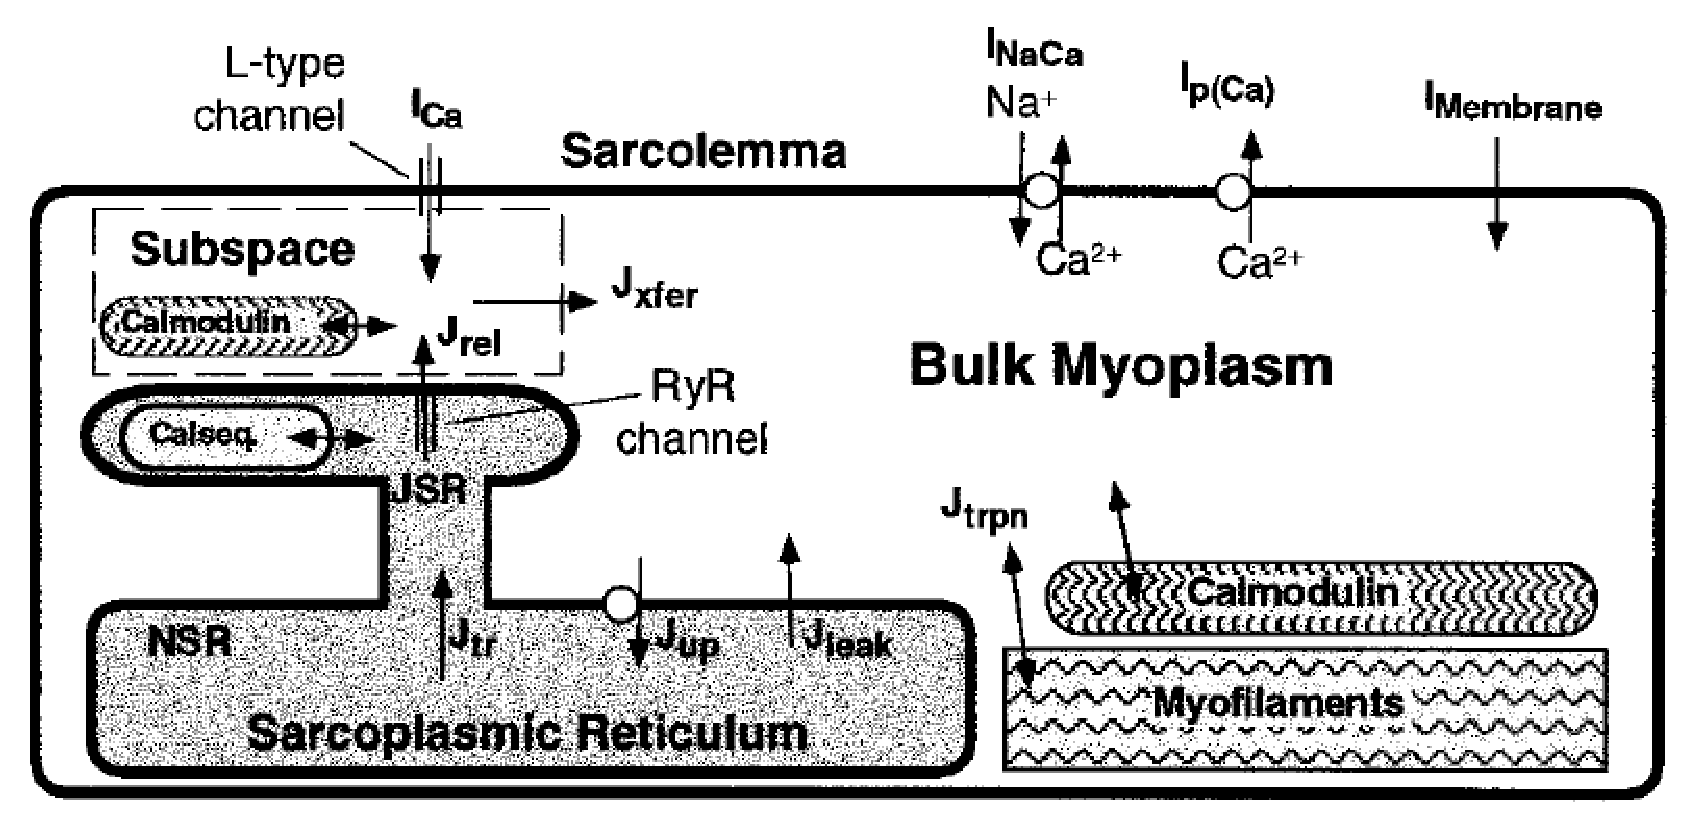
\includegraphics[height=5cm]{./images/buffer_myocyte_diagram.eps}}
  \caption{The diagram of mechanism involving in the dynamics of $\Ca$}
  \label{fig:buffer_Ca}
\end{figure}

In the subspace, calmodulin is the buffer to sequester
$\Ca$. Calsequestrin is the most abundant SR luminal $\Ca$-binding
protein and is found to be in junctional SR, not in network
SR\citep{jafri1998cad}
\begin{equation}
  \label{eq:245}
  B + \ce{Ca^2+ <=> BCa^2+}
\end{equation}
Calsequestrin and calmodulin are considered to be fast buffers, based
on their rate constants. Further, both the high- and low-affinity
sites for troponin are used in this model as calcium-binding sites as
well.

Here, the L-type DHPR channels are neglected; thus, many of the
quantities are avoided, e.g $J_{dhpr}, ...$. As a result,
eq.~\eqref{eq:215} becomes
\begin{equation}
  \label{eq:246}
  \begin{split}
    \overline{c^i_{ds,0}} &= \frac{
      v^T_{efflux}c_{myo}}{\gamma^i_{ryr} v^T_{ryr} + v^T_{efflux}} \\
    \overline{c^i_{ds,1}} &=
    \frac{\gamma^i_{ryr}v^T_{ryr}}{\gamma^i_{ryr} v^T_{ryr} + v^T_{efflux}
    } \\
  \end{split}
\end{equation}


{\bf The fluxes}:
The SERCA-type Ca-ATPase flux is
\begin{equation}
  \label{eq:1900}
  J_{SERCA} = v_{SERCA} \frac{\left( \frac{c_{myo}}{K_{fs}}
    \right)^{\eta_{fs}} - \left( \frac{c_{nsr}}{K_{rs}}
    \right)^{\eta_{rs}}} {1 + \left( \frac{c_{myo}}{K_{fs}}
    \right)^{\eta_{fs}} + \left( \frac{c_{nsr}}{K_{rs}} \right)^{\eta_{rs}}}
\end{equation}
with parameters are constants given in Table 3 of the paper.

The leak $\Ca$ flux is
\begin{equation}
  \label{eq:1910}
  J_{leak} = v_{leak} (c_{nsr}-c_{myo})
\end{equation}
with parameters are experimental-chosen constants.


\section{Ultra-fast Markov-Chain MC method}
\label{sec:ultra-fast-markov}


\section{Numerical stability}
\label{sec:numerical-stability}

A cell model is a set of ODEs and/or PDEs with factors are rate
functions or cellular parameters.  In computational models, when the
membrane potential reaches very high value, e.g. in simulating
defibrillation, it may cause issues with numerical stability. In such
cases, we need to use an extremely small time step. That's why $dV/dt$
is often the criteria being used in adaptive time step approach. To
improve the speed, by retaining the large time step, different
approaches are given:
\begin{enumerate}
\item cut off the rate functions above a certain
  threshold~\citep{skouibine2000}, and intracellular calcium
  concentration is simply held at a constant level for membrane
  potential above a certain threshold, to avoid numerical difficulties
  that can lead to negative concentration values.
\item based on operator splitting, which split the non-linear PDE into
  linear PDEs and a system of non-linear ODEs~\citep{hanslien2007}
\end{enumerate}

\section{Stochastic Petri nets (SPN)}
\label{sec:SPN}

The main limitation of Petri net on practical application is the so-called {\bf
``state-space explosion problem''}. There are different solutions
\begin{enumerate}
  \item ``Kronecker-based'' or ``structure'' method (Sect.\ref{sec:kronecker-based})
\end{enumerate}

The two subsclasses of SPNs are: Superposed Stochastic Automata Network and
Superposed Generalized Stochastic Petri Nets (SGSPN).

\subsection{Superposed Stochastic Automata Network}
\label{sec:superposed_SAN}

Superposed Stochastic Automata Network is a simple subset of Stochastic Petri
Net \citep{donatelli1993,donatelli1994}. Here, solving probability vector $\pi$
can be found \citep{buchholz1992, donatelli1993, donatelli1994, buchholz1995}. 

Superposed stochastic automata network is inspired by the work of Plateau on
Stochastic Automata Network (SAN) (Sect.\ref{sec:SAN}). 

\subsection{Superposed Generalized Stochastic Petri Nets (SGSPN)}
\label{sec:SGSPN}

Superposed Generalized Stochatic Petri Nets (SGSPN) 
\citep{donatelli1994,kemper1996,kemper1996thesis}. Using certain Cartesian
product of reachable states of components is performed, leading to a product
space $\mathbf{\hat{S}}$ that include only actual {\it reachability set}
$\mathbf{S}$. 


\section{Kronecker-based algebra}
\label{sec:kronecker-based}

The Kronecker product is denoted as $\otimes$.
\begin{equation}
\mathbf{C = A \otimes B}
\end{equation}
with $\mathbf{A}\in \mathcal{R}^{n\times m}$, $\mathbf{B}\in
\mathcal{R}^{p\times q}$, $\mathbf{C}\in \mathcal{R}^{(n.p)\times (m.q)}$
\begin{equation}
c_{i,j} = a_{i_1,j_1}b_{i_2j_2}
\end{equation}
with $i = (i_1).p + i_2$ and $j=i_2.q+j_2$. This can be easily extended to
Kronecker product of K matrices:
\begin{equation}
\mathbf{A} = \otimes^K_{k=1} \mathbf{A}^k
\end{equation}
with $A^k \in \mathcal{R}^{n_k\times m_k}$. 

The Kronecker sum is defined only for square matrix. The symbol is $\oplus$. 
\begin{equation}
\mathbf{D = A \oplus B = A \otimes I_p + I_n \otimes B}
\end{equation}
with $\mathbf{A}\in \mathcal{R}^{n\times n}$, $\mathbf{B}\in
\mathcal{R}^{p\times p}$, $\mathbf{D}\in \mathcal{R}^{(n.p)\times (n.p)}$; and
$I_x$ is the identity matrix. The generalization to K matrices is easy
\begin{equation}
\mathbf{A = \sum_{k=1}^K I_{n_1^{k-1}}} \otimes \mathbf{A}^k \otimes
I_{n^K_{k+1}}
\end{equation} 


\begin{framed}
To address a line (column) in the product matrix, we use the so-called {\bf
mixed-based} numbering scheme. $\overline{i}=(i_1,\ldots,i_K)$ correspond to the
number $(\ldots((i_1)n_2 + i_2)n_3)n_K+ i_K$. 
\end{framed}


Kronecker algebra was introduced into the Petri net world in the context of {\it
exact solution of a stochastic model} \citep{donatelli2001}. Here, the
infinitesimal generator {\bf Q} matrix of an SPN is represented via a number of
component $\mathbf{Q}_i$ matrices with $\mathbf{Q}_i$ are generated from $i$-th
submodel (component, subnet) of smaller state space. Using Kronecker operator,
we can generate $\mathbf{Q}$ from $\mathbf{Q}_i$.

There are two situations: 
\begin{enumerate}
  \item  A system is composed of submodels, say $M_1$ and $M_2$. Each is composed
  of a set of reachable states $S^1$ and $S^2$ with finite number of state $n_1$
  and $n_2$, respectively. The global model $\mathcal{M}$ is obtained by the parallel and
  independent composition of the two models. So the global state
  $\overline{i}=(i_1,i_2)$ is represented using mixed-scheme numbering, i.e. 
  $i=i_1.n_2 + i_2$. 
  
If we have K submodels $M_k$, each with state space $S^k$ of $n_k$ states. The
state space of the model $M$ is obtained by the independent parallel composition
of the K models, i.e. the Cartersian product of the state spaces
\begin{equation}
S = S^1 \times \ldots S^K
\end{equation}
and the number of states is $n = |S| = \Pi_{k=1}^K n_k$ \citep{donatelli2001}.
 
$\mathbf{A}, \mathbf{B}$ are square matrices; then they are interpreted
  as state transition matrices of two discrete time Markov chains. So, when the
  global system moves from $\overline{i}=(i_1,\ldots,i_K)$ to
  $\overline{j}=(j_1,\ldots,j_K)$, each component $k$ move from $i_k$ to $j_k$
  at the same time step. The probability for this global state transition is the
  product of the probabilities of the local moves. 
  
    \item What if the system is composed of multiple submodels, but only one is
    allowed to change at a time. Then, this is the case for Kronecker sum
    $\mathbf{D = A \oplus B}$. The first submodel moves, at the same time, the
    second one doesn't move ($\mathbf{A\times I_p}$) or vice versa ($\mathbf{I_n
    \otimes B}$). In this situation, from state $\overline{i} = (i_1,\ldots,
    i_K))$, a candidate for next state $\overline{j} = (j_1,\ldots,j_K)$ only if
    it exists one and only one index $k$ such that $i_k \ne j_k$. 
    
\end{enumerate}

With $\mathbf{Q}$, we need to find the probability transition vector
$\mathbf{pi}$, such that $\mathbf{\pi.Q} = 0$ and $\sum \pi_i = 1$. Early
methods need to explicitly generate $\mathbf{Q}$ and calculate characteristic
steady-state solution $\pi$. Gaussian elimination was used; and the
approximation methods like iterations was used. However, the bootleneck is the
state-space explosion. 

Newer methods can find $\mathbf{pi}$ without computing and storing $\mathbf{Q}$.
Methods of this type are based on superposed stochatic automata network
(Sect.\ref{sec:superposed_SAN}) and SGSPN (Sect.\ref{sec:SGSPN}). Here, the
bottleneck is moved from infinitesimal generator matrix $\mathbf{Q}$ to the
probability vector $\mathbf{\pi}$. 

For matrix-vector multiplication, the idea is that $(K-1)$ additional
multiplications is used instead of generating the full $\mathbf{Q}$ matrix.
Here, only $(K-1)$ additional multiplications is used; or we can use the
so-called
    {shuffle method} which examine sequentially $\mathbf{A}^k$ matrices, one at
    a time \citep{davio1981} (Sect.\ref{sec:shuffle_method}). 

\begin{framed}
Using K component matrices of size $n_k\times n_k$, instead of a single matrix
of size $n\times n$ with $n=\Pi_{k=1}^K$, it has a great advantage of memory
usage. 

Consider the case {\it ordinary} is when the full $\mathbf{Q}$ matrix is
calculated and stored in memory, {\it Shuffle} that use shuffled based equation
and {\it row} which doesn't store $\mathbf{Q}$ but compute each element of the
matrix ``on-the-fly'' when it is needed which implies in theory $K$ additional
multiplication per element \citep{donatelli2001}. 
\begin{itemize}
  \item If $\mathbf{Q}_i$ are stored in full storage, the complexity is
  \item If $\mathbf{Q}_i$ are stored in sparse storage and are ``not too sparse''
  
\end{itemize}
Depending on the sparsity of the matrix, typically {\it shuffle} does better. If
the matrices are ultrasparse, i.e. most row have no or one non-zero, then the
complexity of shuffle and row methods become
\begin{equation}
\bigO(K.n) = \bigO\left( K.\Pi_{k=1}^K\eta(\mathbf{A}^k) \right) = \bigO
(K.\eta(\mathbf{A}))
\end{equation}
\end{framed}
	

\subsection{Shuffle method}
\label{sec:shuffle_method}

Shuffle method was discussed by \citep{davio1981}. Its complexity for the full
storage case was discussed by \citep{steward1994}, and sparse case
\citep{buchholz2000}. 


\section{Stochastic Automata Network (SAN)}
\label{sec:SAN}

Stochastic Automata Network was first developed by Plateau
\citep{plateau1985,plateau1991}.  The idea was then first applied to superposed
stochastic automata (Sect.\ref{sec:superposed_SAN}), and then on a larger
superposed generalized stochastic petri net (SGSPN) 


\section{Tools/Softwares}

For more tools, check Chap.\ref{chap:software-modeling-Neurons}.

\subsection{VirtualCell}
\label{sec:VirtualCell-Tour}

This is a non-continued tool of modeling
\url{http://www.ibiblio.org/virtualcell/}

\subsection{VirtualHeart}

\url{http://thevirtualheart.org/}

%%% Local Variables: 
%%% mode: latex
%%% TeX-master: "mainfile"
%%% End: 
